\documentclass[preview=true]{standalone}
\usepackage{tikz}
\usepackage{pgfplots}
\usepackage[siunitx, american]{circuitikz}
\usepackage[utf8]{inputenc}
\usepackage{newtxtext,newtxmath}
\usepackage[T1]{fontenc}
\pgfplotsset{compat=1.18}
\usepgfplotslibrary{units, fillbetween, smithchart, colormaps}
\usetikzlibrary{positioning, shapes, arrows, arrows.meta, graphs, shapes.geometric, math}
\tikzset{>=latex} % Better arrow tips

\begin{document}
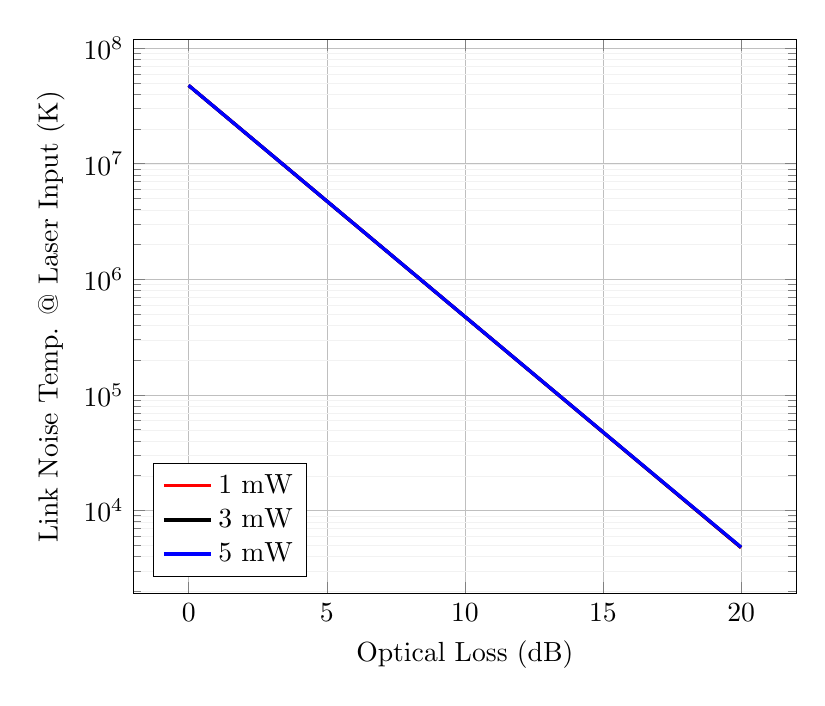
\begin{tikzpicture}[
    declare function={
        RIN(\P) = 10^(-168/10) / \P^2;
        Te(\P,\GOPT,\RS) = 50/(\KB)*(2*\Q*\P*\GOPT*\ETAP + RIN(\P)*\ETAP^2*\GOPT^2*\P^2);
    },
]

\newcommand\KB{1.380649e-23}
\newcommand\Q{1.60217663e-19}
%\newcommand\RIN{3.162278e-15} %-145
\newcommand\ETAP{0.91}
\newcommand\SL{0.22}
\newcommand\RL{5}

\begin{axis}[width={10cm}, 
            grid={both}, 
            grid style={line width={.1pt}, 
            draw={gray!10}}, 
            major grid style={line width={.2pt}, draw={gray!50}},
            ymode=log,
            %ymin = 1000,
            legend pos={south west},
            ylabel={Link Noise Temp. @ Laser Input (K)},
            xlabel={Optical Loss (dB)}]

    \addplot[color=red,
             domain=0:20, 
             samples=100,
             very thick]
    {
      Te(1e-3,10^(-x/10),50)
    };
    \addlegendentry{1 mW}
    \addplot[color=black,
             domain=0:20, 
             samples=100,
             very thick]
    {
      Te(3e-3,10^(-x/10),50)
    };
    \addlegendentry{3 mW}
    \addplot[color=blue,
             domain=0:20, 
             samples=100,
             very thick]
    {
     Te(5e-3,10^(-x/10),50)
    };
    \addlegendentry{5 mW}
            
\end{axis}
\end{tikzpicture}
\end{document}